\chapter{PROBLEM FORMULATION} \label{ProblemFormulation}

The independent use of electric power grids and wireless media for data communication purpose has been pursued since long time ago. However, the need for maximizing their usage and fulfilling the astonishing and growing demands for connectivity among human beings and machines has brought attention to the drawbacks and limitations of these media. Attempting to address these issues, the investigation of the combined use of electric power grids and wireless media for data communication has started a few years ago. 

Currently, an increasing number of works are investigating, characterizing, and modeling hybrid \ac{PLC} and \ac{WLC} channels for improving the performance of in-home broadband communication systems \cite{GalliUS,Canete:Model,Thiago:Characterization,thiago:hyb,thiago:hyb2}. The motivation behind these research effort refers to the need for increasing the reliability, data rate, flexibility and coverage of data communication systems that must fulfill the needs and demands related to the \ac{IoT}, Smart Grids and Indutry $4.0$.
The majority of the aforementioned works adopts well-known channel models in which \ac{PLC} and hybrid \ac{PLC} and \ac{WLC} \acp{CFR} are flat and its \ac{CIR} are modeled as discrete-time and stationary random process. Nevertheless, surveys about electric power grid measurements available in the literature have shown that more investigations have to be carried out to come up with representative \ac{PLC} channel models. In fact, the evolving characteristic and the diversity of loads connected to the electric power systems emphasizes the need for carrying out worldwide measurement campaigns and characterization of electric power systems, mainly in the medium and low-voltage levels. 

Aiming to fulfill this gap,  \cite{Thiago:Characterization,thiago:hyb,thiago:hyb2} discussed measurement campaign and characterization of Brazilian in-home \ac{PLC} and hybrid \ac{PLC}-\ac{WLC} channels over the frequency band from $1.7$ up to $100$~MHz. Based on a extensive measurement campaign carried out in seven Brazilian residences, the characterization of these type of channels were performed over a data set constituted by several \ac{PLC} and hybrid \ac{PLC}-\ac{WLC} channels estimates together with additive noise measurements. A contribution to be added to those presented in \cite{Thiago:Characterization,thiago:hyb} is to provide statistical models of the \ac{CFR}, in order to feed the specifications that researchers need for carrying out more analyses of the data communication systems.

In this regard, this chapter approaches the problem formulation for modeling the \acp{CFR} of the in-home \ac{PLC} and hybrid \ac{PLC}-\ac{WLC} channels, covering the frequency band delimited by $0$ and $B$~Hz . First, a formulation of the broadband \ac{PLC} system is considered with the objective of deriving a concise model for the frequency response of inhome \ac{PLC} channels. In the sequel, a formulation for the hybrid \ac{PLC}-\ac{WLC} system, taking into account the findings reported in \cite{thiago:hyb}, is presented to come up with the statistical model of \ac{CFR} of \ac{PLC}-\ac{WLC} channels, which encompasses the two data communication media (\ac{PLC} and \ac{WLC}).

This chapter is organized as follows: Section \ref{sec:PF1} outlines the problem formulation for the inhome \ac{PLC} channel. In the sequel, Section \ref{sec:PF2} presents the problem formulation the hybrid \ac{PLC}-\ac{WLC} channels. Section \ref{sec:PF3} exposes the investigation questions regarding the formulations presented in Sections \ref{sec:PF1} and \ref{sec:PF2}. Section \ref{sec:PF4} addresses a brief summary on this chapter.

%%%%%%%%%%%%%%%%%%%%%%%%%%%%%%%%%%%%%%%%%%%%%%
\section{PLC CHANNEL} \label{sec:PF1}
%%%%%%%%%%%%%%%%%%%%%%%%%%%%%%%%%%%%%%%%%%%%%%

Fig. \ref{PLCchannel} shows the block diagram of a \ac{PLC} system which is supposed to transmit information carrying signals through an electric power circuit in the frequency band delimited by $0$ and $B$~Hz (i.e., baseband data communication). This electric power circuit is supposed to be linear and time-varying system. According to this figure, the received signal is expressed as
\begin{equation} \label{received signal}
Y_P(t) = \tilde{Y}_P(t)+V_P(t) = \int_{-\infty}^{+\infty} h_P(t,\tau) X(\tau) d\tau + V_P(t),
\end{equation}
where $X(t)\in \mathbb{R}$ is the transmitted signal modeled as a wide sense stationary stochastic process; $h_P(t,\tau)\in \mathbb{R}$ is the time varying \ac{CIR}, related to an impulse applied on the \ac{PLC} channel at the instant $\tau$, modeling the propagation of the transmitted signal through the electric power circuit; $V_P(t)\in \mathbb{R}$ is the additive noise that is modeled as a wide sense stationary random process, $\tilde{Y}_P(t)\in \mathbb{R}$ and $Y_P(t)\in \mathbb{R}$ denote wide sense stationary random processes called the free-of-noise received signal and the received signal, respectively.

\begin{figure}[h]
	\centering
	\psfrag{A}[c][c][1]{Transmitter}
	\psfrag{B}[c][c][1]{PLC Channel}
	\psfrag{C}[c][c][1]{Receiver}
	\psfrag{D}[c][c][1]{$T_X$}
	\psfrag{E}[c][c][1]{$X(t)$}
	\psfrag{F}[c][c][1]{$h_P(t,\tau)$}
	\psfrag{G}[c][c][1]{$\tilde{Y}_P(t)$}
	\psfrag{H}[c][c][1]{$V_P(t)$}
	\psfrag{I}[c][c][1]{$Y_P(t)$}
	\psfrag{J}[c][c][1]{$R_X$}
	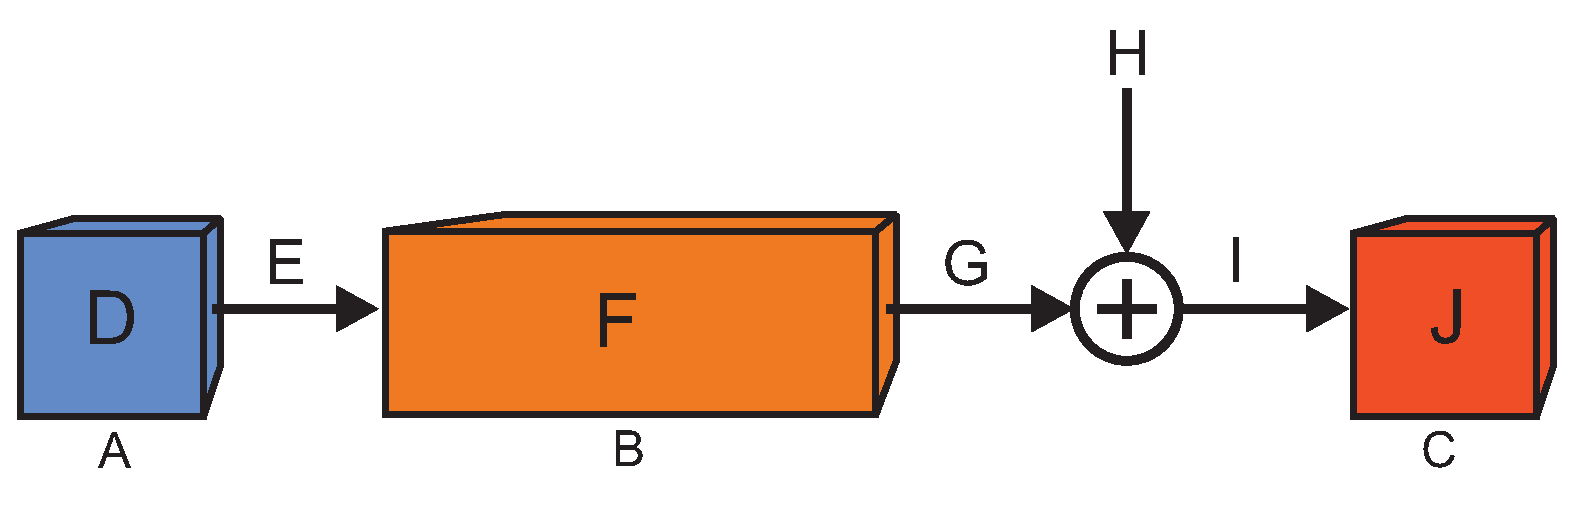
\includegraphics[width=0.9\textwidth]{images/PLCchannel.eps}
	\caption{The block diagram of a PLC system.}
	\label{PLCchannel}
\end{figure}

Due to the \ac{LPTV} behavior of \ac{PLC} channels, which is related to the loads dynamics and the fact that electric power systems transmit or deliver energy at $50$ or $60$~Hz, $h_P(t,\tau)$ can be considered as a cyclostationary stochastic random process with a period equal to a half of the mains frequency \cite{Colen:TCRA}. Based on the knowledge of the coherence time, $T_c \in \mathbb{R}_+$, of the \ac{PLC} channels, the mains cycle ($50$~Hz or $60$~Hz) can be divided into microslots of time interval duration equal to $T_m\in \mathbb{R}_+|T_m < T_c$ and, as a consequence, the \ac{PLC} channels can be modeled as \ac{LTI} during the time interval duration of one microslot. In other words, the channel impulse response of a \ac{PLC} channel at the $i^{th}$ microslot can be expressed as
\begin{equation} \label{discreteh}
h_{i}(t),~\forall~t \in [iT_{m}, (i+1)T_{m}] \mid T_{m} < T_{c}.
\end{equation}
From now on, we drop the index $i$ for facilitating further deductions. Based on this adoption, the discrete-time representation of the \ac{CIR} of the \ac{PLC} channel in a microslot is given by
\begin{equation} \label{discreteCFR}
h[n] = h_P(t)|_{t=nT_s} , n = 0,1, \ldots, L_h-1, 
\end{equation}
where $L_{h}$ is the length of the \ac{LTI} \ac{PLC} channel, $T_s=1/f_s$ is the sampling period and $f_s=2B$~Hz is the sampling frequency. Usually, the value of $L_{h}$ contribute to the adoption of an \ac{HS-OFDM} scheme for channel estimation because the number of subcarriers of an \ac{HS-OFDM} symbol ($2N$) is chosen to ensure that $2N \gg L_h$. Moreover, $B/N < B_c$, in which $B_c$ is the coherence bandwidth of the \ac{PLC} channels. In order to work with $2N$ subcarriers in the \ac{HS-OFDM} scheme for performing \ac{CFR} estimation, the zero-padding have to be applied to $\{h[n]\}$. In vectorial terms, let ${\bf h}=[h_0 h_1 \ldots h_{L_h-1}]^T$, such as $h_n=h[n]$, then we can obtain an $2N\text{-length}$~vector (i.e., $N\in \mathbb{N}|B/N<B_c$) that represents the extended version of the vector ${\bf h}$ when the zero-padding approach is taken into account. As a consequence, the vectorial representation of the \ac{CFR} associated with the extended version of the vector $\mathbf{h}$ is expressed as

\begin{equation}
\mathbf{H} = \mathbf{W}_{2N}  \begin{bmatrix} \mathbf{I}_{L_h} \\ \mathbf{0}_{(2N-L_{h})\times L_{h}} \end{bmatrix} \mathbf{h},
\end{equation}
where $\mathbf{W}_{2N} \in \mathbb{C}^{2N\times 2N}$ denotes the $2N \times 2N$-size \ac{DFT} matrix, $ \mathbf{I}_{L_h} \in \mathbb{R}^{L_h\times L_h}$ denotes an $L_h\times L_h$-size identity matrix, and $ \mathbf{0}_{(2N-L_{h})\times L_{h}} $ is an $ (2N-L_{h})\times L_{h}$ null matrix. The $k^{th}$ element of the vector $\mathbf{H}=[H_0 H_1 \ldots H_{2N-1}]^T \in \mathbb{C}^{2N\times 1}$ may be expressed in polar form $H_k=|H_k|\exp(j \Theta_k)$, in which $|.|$ denotes the absolute value and $\Theta_k$ is the phase value of $H_k$. Since the \ac{CIR} of the \ac{PLC} channel is real-valued, it means that \ac{CFR} posses the hermitian symmetry property and, as a consequence, only the first half of samples of the \ac{CFR} have to be analyzed. The vectors $|{\bf H}|\triangleq [|H_0||H_1|\ldots |H_{N-1}|]^T$ and ${\bf \Theta}\triangleq[\Theta_0\Theta_1\ldots \Theta_{N-1}]^T$ are two distinct random processes that represent, respectively, the magnitude and phase of the first half of the vector $\mathbf{H}$. The modeling of \ac{CFR} based on these two vectors is very useful for data communication purpose once that the knowledge of the magnitude and the squared magnitude (i.e.,  $|{\bf H}|^2\triangleq[|H_0|^2|H_1|^2\ldots |H_{N-1}|^2]^T$) of the \ac{CFR} allows deriving closed-form expression of theoretical channel capacity, energy harvesting, physical layer security, among other things. Also, the knowledge of phase allows the derivation of delay spread and group delay. It is important to emphasize that the nature of \ac{PLC} channels indicates that the vectors $|{\bf H}|$ and ${\bf \Theta}$ are non-stationary and correlated random processes. 
 
Since the vector $\mathbf{H}$ is a \ac{r.v.} that can be represented by the  two distinct \acp{r.v.} (i.e., $|{\bf H}|$ and ${\bf \Theta}$), a generic \ac{r.v.} $\bf X\in\{|H|,\Theta\}$ is adopted. Therefore, we assume that the $k^{th}$ \ac{r.va.} belonging to both random processes (i.e., the element $|H_k|$ or $\Theta_k$) can be modeled by an statistical distribution owing a set of parameters represented by $\mathcal{C}_{X_k} = \{ \zeta_{1}[k], \cdots, \zeta_{U}[k] \}$, which is constituted by $U \in \mathbb{N}_+$ parameters. Note that $\zeta_{u}[k] \in \mathbb{R}$ is the $u^{th}$ parameter associated with the chosen statistical distribution offering the best description of the $k^{th}$ element of the \ac{r.v.} $\bf X$ (i.e., $|{\bf H}|$ or ${\bf \Theta}$).

%%%%%%%%%%%%%%%%%%%%%%%%%%%%%%%%%%%%%%%%%%%%%%
\section{HYBRID PLC-WLC CHANNEL} \label{sec:PF2}
%%%%%%%%%%%%%%%%%%%%%%%%%%%%%%%%%%%%%%%%%%%%%%

Fig. \ref{Hybchannel} shows the block diagram of the employment of hybridism concept in a data communication system, in which \ac{PLC} and \ac{WLC} channels are employed in cascade
without an intermediate data communication node between them.. As a matter of fact, \ac{PLC} devices are connected to electric power grids through a coupling circuit while the \ac{WLC} devices are connected to the air through an antenna. The \ac{PLC} and \ac{WLC} devices directly communicate with each other since both of them occupy the frequency band delimited by $0$ and $B$~Hz. 

According to \cite{thiago:hyb}, as the signal transmitted by a \ac{PLC} device is irradiated from unshielded power lines, a \ac{WLC} device can be  wirelessly connected to a \ac{PLC} system, which is supposed to work with \ac{PLC} devices physically connected to power lines. Similarly to Section \ref{sec:PF1}, the received signals at the input of the hybrid \ac{PLC}-\ac{WLC} channels, which is supposed to be a linear stochastic system, are expressed as
\begin{equation} \label{received signal2}
Y_{PW}(t) = \int_{-\infty}^{+\infty} h_{PW}(t,\tau) X(\tau) d\tau + V_{PW}(t),
\end{equation}
for the signal propagation from the \ac{PLC} device to the \ac{WLC} device (i.e., \ac{PLC}~$\rightarrow$~\ac{WLC} direction), and
\begin{equation} \label{received signal3}
Y_{WP}(t) = \int_{-\infty}^{+\infty} h_{WP}(t,\tau) X(\tau) d\tau + V_{WP}(t),
\end{equation}
for the reverse path, which is defined by the signal propagation from the \ac{WLC} device to the \ac{PLC} device (i.e., \ac{WLC}~$\rightarrow$~\ac{PLC} direction). In (\ref{received signal2})-(\ref{received signal3}),  $X(t)\in \mathbb{R}$ is the transmitted signal modeled as a wide sense stationary stochastic process; $h_{PW}(t,\tau)\in \mathbb{R}$ and $h_{WP}(t,\tau)\in \mathbb{R}$ denote the \acp{CIR} when an impulse at the instant $\tau$ is applied to the \ac{PLC}~$\rightarrow$~\ac{WLC} and \ac{WLC}~$\rightarrow$~\ac{PLC} directions, respectively; $V_{PW}(t)\in \mathbb{R}$ and $V_{WP}(t)\in \mathbb{R}$ are, respectively, the additive noise components and are modeled as two different wide sense stationary random processes found at the input of the transmitting transceivers, when the \ac{PLC}~$\rightarrow$~\ac{WLC} and \ac{WLC}~$\rightarrow$~\ac{PLC} directions, respectively, take place; $Y_{PW}(t)\in \mathbb{R}$ and ${Y}_{WP}(t)\in \mathbb{R}$ are wide sense stationary random processes denoting the received signals, respectively, in the \ac{PLC}~$\rightarrow$~\ac{WLC} and \ac{WLC}~$\rightarrow$~\ac{PLC} directions.

\begin{figure}[h]
	\centering
	\psfrag{A}[c][c][1]{Wall}
	\psfrag{B}[c][c][1]{hybrid-PLC}
	\psfrag{C}[c][c][1]{Transceiver}
	\psfrag{D}[c][c][1]{PLC coupler}
	\psfrag{E}[c][c][1]{Power}
	\psfrag{F}[c][c][1]{line}
	\psfrag{G}[c][c][1]{PLC signal}
	\psfrag{H}[c][c][1]{hybrid-Wireless}
	\psfrag{I}[c][c][1]{Transceiver}
	\psfrag{J}[c][c][1]{Antenna}
	\psfrag{K}[c][c][1]{Wireless}
	\psfrag{L}[c][c][1]{signal}
	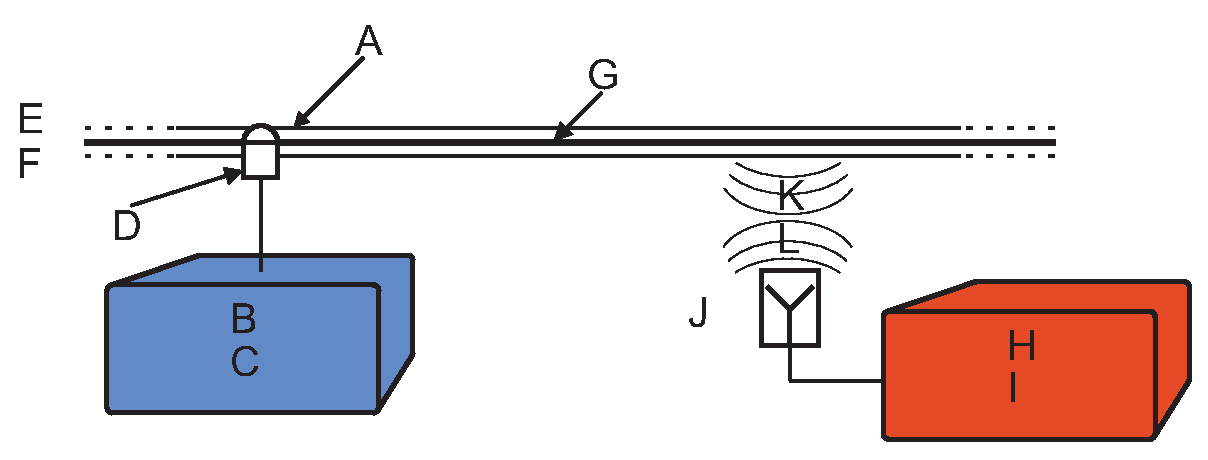
\includegraphics[width=0.9\textwidth]{images/Hybrid_channel.eps}
	\caption{The block diagram of a hybrid PLC-WLC system.}
	\label{Hybchannel}
\end{figure}

It is important to highlight that the symmetry of the hybrid \ac{PLC}-\ac{WLC} channel magnitude response is verified when the transmitter and the receiver have the same access impedance, see \cite{thiago:hyb}. In other words, the \ac{CFR} of the hybrid \ac{PLC}-\ac{WLC} channel remains the same independent from the data transmission direction. Mathematically, $h_{PW}(t,\tau)=h_{WP}(t,\tau)$ agrees with the results presented in \cite{Galli:indoor}, which focuses only on \ac{PLC} channels. Due to the specific characteristics of each media (e.g., power line and air), the symmetry properity does not hold true for the additive noises $V_{PW}(t)$ and $V_{WP}(t)$ \cite{thiago:hyb}. As a matter of fact the additive noise in a power line is constituted by several components that are generated by dynamic of load connected to electric power grids. It is well-known as man-made-noise and present a power spectral density that exponentially decay as frequency changes from $0$~Hz to $30$~MHz. On the other hand, the  noise in the air considering the frequency band between $0$ and $100$~MHz owns a almost constant power spectral density with some peaks that are associated with narrowband channels dedicated to AM and FM stations, among others. The findings reported in \cite{thiago:hyb,thiago:hyb2,thiago:doc} are very interesting to motivate this kind of data communication systems for fulfilling the scarcity of spectrum for dealing with te astonishing increase of data exchanges among entities in smart grids, the \ac{IoT} and industry $4.0$ applications. Advances in this field may facilitate the work of researchers and hybrid \ac{PLC}-\ac{WLC} systems designers under the availability and representative of hybrid \ac{PLC}-\ac{WLC} channels. 
    
In \cite{thiago:hyb} was proposed the following organization for modeling the hybrid \ac{PLC}-\ac{WLC} channels:
    
\begin{itemize}
\item \textit{short-path} channel: On this scenario, the \ac{WLC} Transceiver may be randomly positioned within a $2$~m radius circle, centered at the outlet in which the \ac{PLC} Transceiver was connected.

\item \textit{long-path} channel: On this scenario, the \ac{WLC} Transceiver was randomly placed into a area defined as a swept circle, having an outer and inner radius of $6$~m and $2$~m, respectively, centered at the outlet in which the \ac{PLC} Transceiver was connected.
\end{itemize}
    
Fig. \ref{hybSL} shows the coverage region related to the \textit{short-path} and \textit{long-path} channels. According to \cite{thiago:hyb,thiago:hyb2,thiago:doc}, these channels are different because the attenuation of the signal remarkably increases with the distance of the \ac{WLC} device from the power line. 

\begin{figure}[h]
	\centering
	\psfrag{A}[c][c][1]{Wall}
	\psfrag{B}[c][c][1]{hybrid-PLC}
	\psfrag{C}[c][c][1]{Transceiver}
	\psfrag{D}[c][c][1]{Outlet}
	\psfrag{E}[c][c][1]{PLC coupler}
	\psfrag{F}[c][c][1]{2-meters}
	\psfrag{G}[c][c][1]{6-meters}
	\psfrag{H}[c][c][1]{hybrid-Wireless}
	\psfrag{I}[c][c][1]{Transceiver}
	\psfrag{J}[c][c][1]{Antenna}
	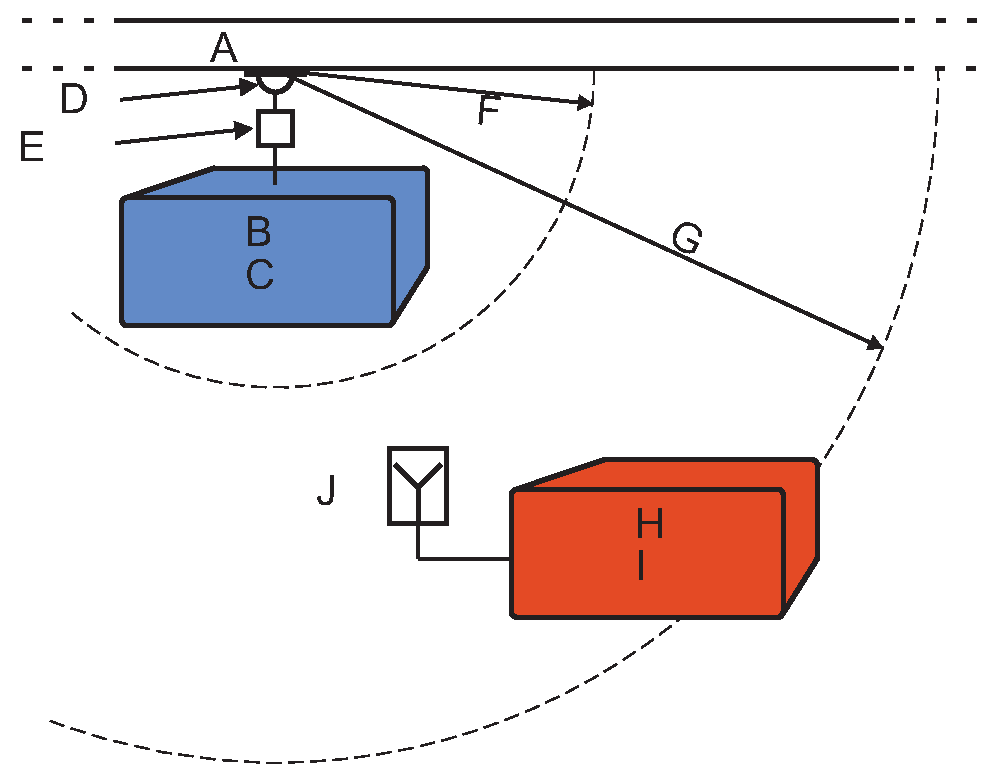
\includegraphics[width=0.9\textwidth]{images/Hybrid_LandS_channel.eps}
	\caption{Measurement setup for the \textit{short-path} (2-m) and \textit{long-path} (6-m) versions of the hybrid PLC-WLC channels.}
	\label{hybSL}
\end{figure}

Similar to \ac{PLC} systems, the hybrid \ac{PLC}-\ac{WLC} system operates in the baseband. Therefore the deduction adopted in Subsection \ref{sec:PF1} is directly applied to the channel impulse responses of the \ac{PLC}-\ac{WLC} channels considering both \textit{short-path} and \textit{long-path} scenarios. As a result, the vectorial representation of channel frequency response of the hybrid \ac{PLC}-\ac{WLC} channel is denoted by the vector ${\bf X} \in \{ |{\bf H}|, {\bf \Theta} \}$. 

%%%%%%%%%%%%%%%%%%%%%%%%%%%%%%%%%%%%%%%%%%
\section{INVESTIGATION QUESTIONS} \label{sec:PF3}
%%%%%%%%%%%%%%%%%%%%%%%%%%%%%%%%%%%%%%%%%%

Given the aforementioned formulation, the following research questions arise regarding the modeling of \acp{CFR} of in-home \ac{PLC} and hybrid \ac{PLC}-\ac{WLC} channels within a time interval corresponding to one microslot: 

\begin{itemize}
	\item \textit{What kind of statistical distributions are suitable for modeling the random variables that constitute the vectors $|{\bf H}|$ and ${\bf \Theta}$ under the availability of measured data set obtained from a measurement campaign carried out in Brazilian residences?}
	\item \textit{Could we state that the random vectors $|{\bf H}|$ and ${\bf \Theta}$ related to the measured \ac{PLC} and hybrid \ac{PLC}-\ac{WLC} channels in Brazilian residences are stationary random processes?}
    \item \textit{Which level of correlations exist among the elements of vectors $|{\bf H}|$ and ${\bf \Theta}$? How to address this feature of  these random processes to come up with a generator of channel frequency responses of in-home \ac{PLC} and hybrid \ac{PLC}-\ac{WLC} channels?}  
\end{itemize}

The first and second research questions are covered in this dissertation, while the third research question is left for being investigated in a future work. The investigation of the first two research questions is very interesting from the data communication perspective because it can offer models for allowing researchers to investigate channel capacity, cooperative communication, energy harvesting, physical layer security, among other things.

Chapters \ref{Proposal} and \ref{NumericalResults} try to answer the first two research questions.

%%%%%%%%%%%%%%%%%%%%%%%%%%%%%%%%%%%%%%%%%%
\section{SUMMARY} \label{sec:PF4}
%%%%%%%%%%%%%%%%%%%%%%%%%%%%%%%%%%%%%%%%%%

This chapter has focused on the formulation of the problems addressed in this thesis. %problem formulation addressing the two aforementioned scenarios of communications (\ac{PLC} and \ac{PLC}/wireless) has been presented. \textcolor{red}{Also a way of modeling the \ac{CFR} of these scenarios was highlighted, based on two random vectors, denoting two random processes, that represent the magnitude and phase component of the \ac{CFR}. This proposed modeling was used in order to characterize both \ac{PLC} and \ac{PLC}/wireless channels \acp{CFR}}.